\documentclass[12pt]{article}
\usepackage[utf8]{inputenc}
\usepackage[T1]{fontenc}
\usepackage{amsfonts, amsmath}
\usepackage{tikz}
\usetikzlibrary{positioning}
\usepackage{xcolor, soul}

\begin{document}

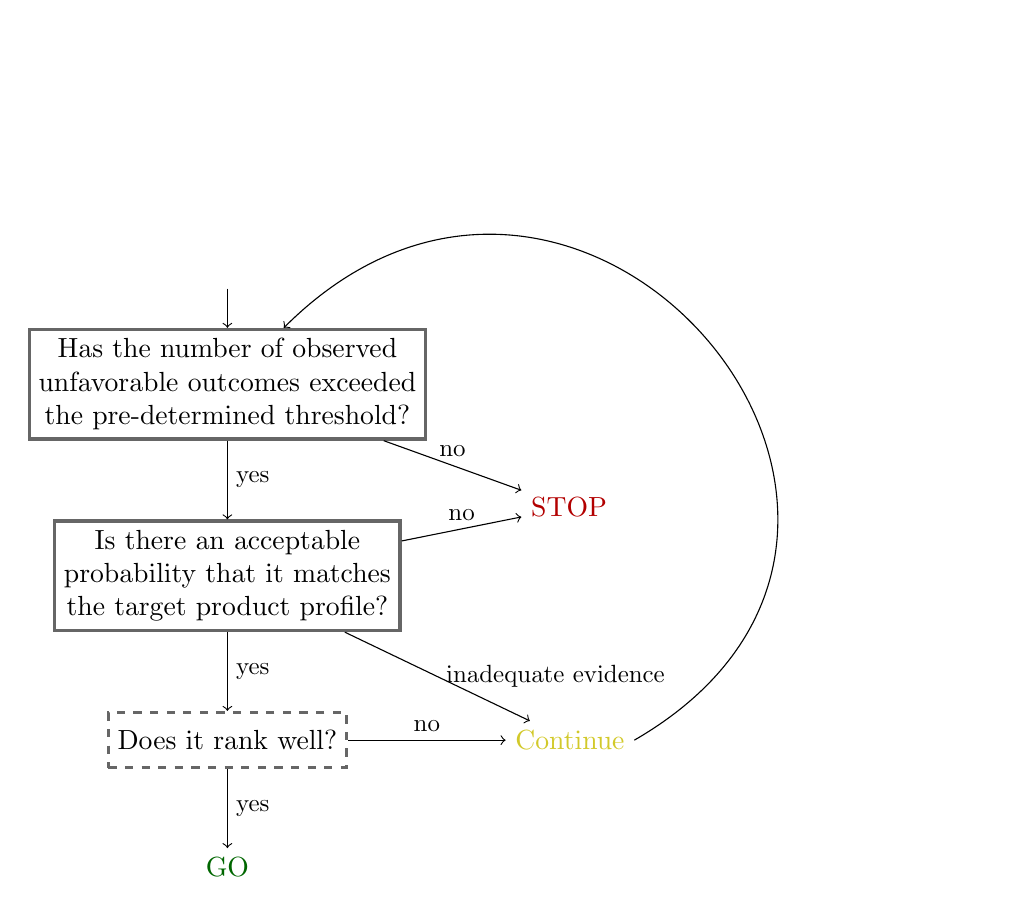
\begin{tikzpicture}[
dashednode/.style={rectangle, draw=black!60, very thick, dashed, minimum size=7mm},
squarednode/.style={rectangle, draw=black!60, very thick, minimum size=5mm},
]
%Nodes
\node[squarednode, align=center]      (q1)               {Has the number of observed\\unfavorable outcomes exceeded\\the pre-determined threshold?};
\node                                 (q0)       [above=0.5cm of q1] {};
\node[squarednode, align=center]      (q2)       [below=of q1] {Is there an acceptable\\probability that it matches\\the target product profile?};
\node[dashednode]                     (q3)       [below=of q2] {Does it rank well?};
\node[black!60!green]                 (go)       [below=of q3] {GO};
\node                                 (temp)     [right= 2cm of q2] {};
\node[black!30!red]                   (stop)     [above= 0.5cm of temp]{STOP};
\node[black!20!yellow]                (continue) [right= 2cm of q3]{Continue};

%Lines
\draw[->] (q0) -- (q1);
\draw[->] (q1) -- node [right,scale=0.9] {yes} (q2);
\draw[->] (q1) -- node [above,scale=0.9] {no} (stop);
\draw[->] (q2) -- node [right,scale=0.9] {yes} (q3);
\draw[->] (q2) -- node [above,scale=0.9] {no} (stop);
\draw[->] (q2) -- node [right,scale=0.9] {inadequate evidence} (continue);
\draw[->] (q3) -- node [right,scale=0.9] {yes} (go);
\draw[->] (q3) -- node [above,scale=0.9] {no} (continue);
\draw[->] (continue.east) to [out=30,in=45,looseness=2] (q1);
\end{tikzpicture}

\end{document}